\chapter{Procedures, Stacks, and ABIs}
\label{ch:procedures-abis}

A machine can transfer control and preserve a continuation without knowing
what a function is. A compiler can place an argument in a register without
changing that register's instruction-set meaning. A procedure emerges when
separately written pieces of code agree about entry, return, values, scratch
space, and preservation.

That agreement is an \keyterm{application binary interface}, or ABI. It sits
between source-language intention and instruction semantics. Confusing the
layers produces brittle explanations: an ISA register gets called an argument
register in every context, a stack-growth convention is mistaken for a
hardware law, or a successful return is credited to \code{RET} while the
saved address and stack discipline go unproved.

\begin{keyidea}[title={A call mechanism is not a calling convention}]
The ISA explains how control reaches a target and how a continuation is
recorded. The ABI explains where arguments and results live, which locations
survive the call, how the stack is aligned, and who restores each resource.
Procedure correctness needs both layers and must name each separately.
\end{keyidea}

\section{Why procedures became a machine-level agreement}

Early programmers quickly learned that repeating instruction sequences by
copying them was costly and error-prone. A reusable subroutine stored one body
and let many sites transfer to it. Reuse created a new problem: the body had
to know where to return, where to find its inputs, where to place its result,
and which working locations belonged to its caller.

Assemblers and languages supplied conventions before those conventions became
large platform documents. Linkers then had to connect separately assembled
objects. Debuggers needed to recover call chains. Operating systems and shared
libraries needed independently produced code to agree for years. The modern
ABI records that durable binary agreement. It covers much more than calls,
but this chapter uses its procedure-calling slice.

The same need exists today in compilers, foreign-function interfaces, dynamic
instrumentation, binary translation, and formal verification. A compiler may
optimize freely inside a procedure while still owing a precise boundary to
every caller. A proof that two function bodies compute the same number is
insufficient if one corrupts a preserved register, misaligns the stack before
a nested call, or returns through the wrong address.

\begin{archive}[title={A procedure boundary makes separate construction possible}]
The caller need not know how the callee computes. The callee need not know why
the caller wants the result. Both must know the narrow contract at the entry
and exit. That controlled ignorance is what permits separate compilation.
\end{archive}

\section{Six parts of a procedure contract}

For one scalar procedure, write the contract as six declarations:

\begin{enumerate}
\item \emph{entry control}: the address and machine state from which the body
begins;
\item \emph{inputs}: registers or memory locations containing arguments;
\item \emph{outputs}: locations containing results on normal return;
\item \emph{volatile state}: scratch locations the caller must assume may
change;
\item \emph{preserved state}: locations the callee must restore before return;
\item \emph{return control}: the saved continuation and rule that resumes it.
\end{enumerate}

Stack bounds, alignment, allowed traps, and memory ownership refine these
parts. The contract also needs an observation: perhaps the result, preserved
registers, stack pointer, reachable memory, and normal-return outcome. It need
not require temporary registers to recover their entry values.

\begin{definition}[title={Caller-saved and callee-saved name obligations}]
A caller-saved location may be overwritten by a conforming callee, so a caller
with a live value there must save it before the call. A callee-saved location
must have its entry value again when the callee returns normally, so a callee
that uses it must save and restore it. Neither term says who physically owns a
register; each assigns a proof obligation at the boundary.
\end{definition}

The two disciplines can implement the same preservation fact. If a value must
survive a call, the caller may move it out of volatile state, or the callee may
promise to preserve its chosen location. Performance, register pressure, and
code size influence the division. Semantics requires only that the printed
contract be met.

\begin{example}[title={A value that is dead needs no ceremony}]
Suppose the caller places a temporary in a volatile register and never reads
it after the call. The callee may overwrite it without a save. If a later edit
makes the value live across the call, the old sequence becomes wrong unless
the caller saves it or moves it to a preserved location. Liveness turns an ABI
permission into a concrete save obligation.
\end{example}

\subsection{A procedure theorem has four layers}

A useful theorem about a procedure is not merely a relation between two
snapshots. It joins four layers of reasoning. The \emph{entry relation}
connects the caller's abstract arguments and resources to concrete machine
locations. A \emph{body invariant} explains why every reachable internal
state remains safe and still has enough information to finish. Each
\emph{call checkpoint} establishes the entry contract of a nested callee and
records what the current procedure must keep across that call. Finally, the
\emph{exit relation} connects the machine state back to the promised result,
preserved resources, and continuation.

\begin{figure}[htbp]
\centering
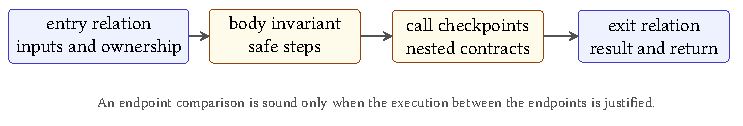
\includegraphics[width=0.94\textwidth]{figures/procedure-contract-layers}
\caption{A procedure proof crosses four layers. Skipping the middle two turns
an endpoint comparison into an assumption about the body.}
\figalt{Four boxes run from entry relation through body invariant and nested-call checkpoints to the exit relation.}
\label{fig:procedure-contract-layers}
\end{figure}

This division prevents a common circular argument. Suppose a test begins in a
valid entry state and happens to finish in a valid exit state. That observation
does not show that all valid entries finish, that intermediate memory accesses
are permitted, or that the body cannot jump somewhere else. The trace or
inductive proof must connect the endpoints. Conversely, a safe trace that
halts at the wrong continuation does not establish the procedure contract.

For a straight-line leaf, the body invariant may be no more than a symbolic
expression for each changed register and a claim that the next instruction is
defined. A loop needs a genuine loop invariant. A non-leaf body needs a
checkpoint before every nested call. The theorem should become larger only
when the control structure becomes larger; the boundary vocabulary remains
the same.

\begin{proofkit}[title={Normal-return procedure theorem schema}]
Assume an entry state satisfies the procedure precondition and entry relation.
Show that each instruction step is defined and preserves the body invariant.
At a nested call, derive the callee's precondition, apply its procedure
theorem, and reestablish the caller's invariant from the callee's exit
relation. At a normal return, derive the result relation, restored stack
pointer, preserved locations, allowed memory effect, and saved continuation.
This establishes only the normal-return behavior named by the theorem; a trap,
divergence, or exceptional exit needs a separate clause.
\end{proofkit}

\section{A stack is memory governed by an invariant}

An architectural stack pointer is an ordinary register with special uses or
conventions. A0 has none. RV64I base instructions do not force \code{x2} to be
a stack pointer; the RISC-V ABI names it \code{sp}. In x86-64, \code{RSP} has
instruction-level roles in \code{CALL}, \code{RET}, \code{PUSH}, and
\code{POP}, while the ABI adds alignment, frame, and preservation rules.

A downward-growing stack allocates a frame by subtracting from the stack
pointer and releases it by adding the same size. ``Downward'' refers to
numerical addresses, not to the way a diagram is drawn. The allocated frame is
a byte range, and every load or store still needs an address, width, byte
order, alignment policy, and range premise.

\begin{figure}[htbp]
\centering
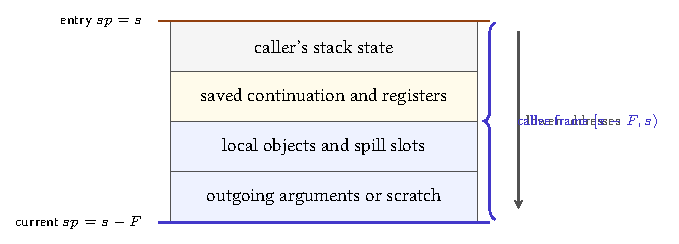
\includegraphics[width=0.72\textwidth]{figures/stack-frame-anatomy}
\caption{A downward-growing frame after allocation. The current stack pointer
marks its low address; the caller's stack state lies at higher addresses.}
\figalt{A vertical memory diagram shows lower addresses below, a callee frame above the stack pointer, and caller state at higher addresses.}
\label{fig:stack-frame-anatomy}
\end{figure}

Let \(s\) be the entry stack pointer and let a callee allocate \(F\) bytes.
After \(sp'=s-F\), its frame occupies the half-open interval
\([
sp',s)
\). A store of \(k\) bytes at address \(a\) stays within the frame exactly
when
\[
  sp'\leq a \quad\hbox{and}\quad a+k\leq s.
\]
The half-open form handles adjacent objects without overlap and makes the
upper-bound proof explicit.

\begin{proofkit}[title={Balanced allocation restores the stack pointer}]
Assume address arithmetic does not wrap and the entry pointer is \(s\).
Allocating \(F\) bytes produces \(s-F\). Releasing the same frame produces
\((s-F)+F=s\). This proves pointer restoration, not frame correctness. A
separate argument must show that every access stayed within allocated and
permitted memory and that every saved value was restored before release.
\end{proofkit}

Alignment is a modular invariant. If the ABI requires alignment \(A\), then a
required checkpoint satisfies \(sp\bmod A=0\). Subtracting a frame size that
is a multiple of \(A\) preserves alignment. A call mechanism that pushes a
return address may deliberately change the congruence observed at callee
entry, so the checkpoint and mechanism must be stated together.

\begin{warning}[title={Balanced arithmetic does not prove a safe frame}]
A prologue and epilogue can restore the same stack-pointer value while writing
outside the frame, overwriting the saved return address, restoring the wrong
register value, or violating alignment at an intervening call. Check the
whole interval and every required checkpoint.
\end{warning}

\subsection{Nested frames are interval arithmetic}

Suppose a procedure enters with stack pointer (s), allocates (F) bytes,
and calls a second procedure that allocates (G) bytes. Immediately before
the nested allocation, the first frame is ([s-F,s)). After it, the nested
frame is ([s-F-G,s-F)). The intervals touch at (s-F) but do not overlap.
This simple calculation is the spatial reason one procedure may keep saved
values in its frame while another procedure uses the stack below it.

\begin{figure}[htbp]
\centering
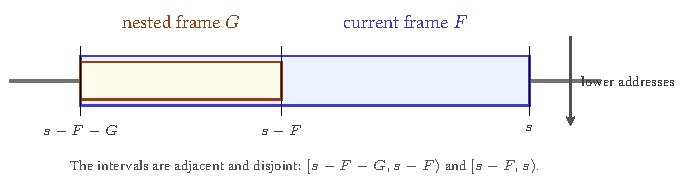
\includegraphics[width=0.86\textwidth]{figures/stack-interval-nesting}
\caption{Nested downward-growing frames as half-open byte intervals. The
orientation of the drawing is secondary; the address inequalities are the
claim.}
\figalt{A horizontal address line shows a nested G-byte frame immediately below a surrounding F-byte frame, with their half-open endpoints labeled.}
\label{fig:stack-interval-nesting}
\end{figure}

The argument depends on more than subtraction. Neither computation may wrap.
Both intervals must lie in mapped, writable memory owned by the stack. The
nested callee must respect its own frame bound rather than store upward into
the caller's frame. If it receives a pointer into the caller's frame, any
write through that pointer must be separately allowed by the contract. Stack
discipline supplies disjoint default regions; explicit pointer sharing can
weaken that separation.

A frame proof is therefore a small memory-safety proof. For each slot, record
an offset, width, alignment, and lifetime. Prove that its interval is inside
the frame and disjoint from every simultaneously live slot unless intentional
aliasing is part of the design. Then prove that the frame as a whole is inside
the permitted stack region. Checking only the largest printed offset misses
the width of the access: an eight-byte store beginning four bytes below the
upper boundary crosses it.

\section{A0 exposes the missing mechanism}

Core A0 has direct relative \code{jump}, conditional branches, and eight
ordinary registers. It has no call instruction, register-indirect jump,
implicit stack pointer, or ABI. That is a useful boundary rather than an
omission to conceal.

A fixed-call-site teaching program can jump directly to a body and let that
body jump directly back to one known continuation. It can designate \(r_6\)
as a stack pointer and \(r_7\) as a saved link by convention. Yet core A0
cannot use an arbitrary value in \(r_7\) as the next program counter. A body
shared by multiple callers therefore needs duplicated return blocks, a
dispatch scheme, self-modifying code outside the model, or an explicit
instruction-set extension.

\begin{sidebar}[title={Do not smuggle a return instruction into A0}]
Writing a return address into \(r_7\) does not make \code{jump r7} legal when
the A0 specification defines only a relative-immediate jump. Examples must
either use a fixed direct return or declare an A0 extension with its own
encoding, semantics, traps, and evidence controls.
\end{sidebar}

This limitation clarifies the construction order. First define a procedure
contract independently of any particular call opcode. Then show a fixed A0
instance satisfying it. If the book later adds an indirect-jump extension,
prove that its general call/return sequence refines the same contract. The
contract survives even as the mechanism becomes richer.

For a fixed-return A0 leaf, choose conventions only for the example: \(r_0\)
holds one input and the result, \(r_6\) is an aligned stack pointer, \(r_4\)
and \(r_5\) are preserved, and \(r_1,r_2,r_3,r_7\) are volatile. The body may
compute without a frame. Its proof must show the result relation, preservation
of \(r_4,r_5,r_6\), permitted scratch changes, unchanged memory, and a direct
jump to the unique continuation.

\section{RV64I separates link register from stack memory}

RV64I \code{JAL} writes \(pc+4\) to a destination register and transfers to a
PC-relative target. The common call convention writes the link to \code{x1},
named \code{ra}. \code{JALR} can transfer to an address computed from a
register and immediate while writing another link. The assembler spelling
\code{ret} denotes the appropriate base-instruction form that jumps through
\code{ra}; it is not a new architectural instruction \autocite{riscv2026unpriv}.

The RV64 integer ABI gives selected registers procedure roles. It names
\code{x2} as \code{sp}, uses \code{a0}--\code{a7} for integer arguments,
uses \code{a0} and \code{a1} for integer return values, classifies
\code{t0}--\code{t6} as temporaries, and requires \code{s0}--\code{s11} to
be preserved. The standard stack grows toward lower addresses and is aligned
to a 128-bit boundary at procedure entry; the standard ABI requires that
alignment through procedure execution \autocite{riscv2026abi}.

Consider a leaf function that adds one to its first integer argument:

\begin{codelisting}[language={},caption={An RV64I leaf under the selected integer ABI}]
add_one:
    addi a0, a0, 1
    jalr x0, 0(ra)
\end{codelisting}

The ISA explains both instructions. The ABI explains why entry \code{a0} is
the argument, exit \code{a0} is the result, \code{ra} contains the caller's
continuation, and no preserved register needs saving. The mathematical
precondition decides whether the desired result is modular addition or
ordinary integer addition without wrap.

A non-leaf function cannot assume \code{ra} will survive its own nested call:
the nested linking jump writes a new continuation there. It must preserve its
incoming return address, often in its stack frame, before making the call and
restore it before returning. That need follows from liveness plus the call
mechanism, not from a rule that every function must have the same prologue.

\begin{tryit}[title={Find the first overwritten continuation}]
Trace a function entered with \code{ra}=100 that immediately calls another
function using \code{jal ra,target}. Record \code{ra} after the nested call.
Explain why a later \code{jalr x0,0(ra)} cannot return to 100 unless the
original value was kept elsewhere and restored.
\end{tryit}

\subsection{Leaf is a control-flow fact, not a size class}

A \keyterm{leaf procedure} makes no procedure call on the path under
discussion. A \keyterm{non-leaf procedure} does. The distinction does not say
that a leaf is short, uses no stack, or cannot loop. A leaf may allocate a
large frame, spill registers, and run for millions of steps. A non-leaf may
contain only a few instructions around one call.

The distinction matters because a leaf can often keep its incoming
continuation in the location established by its caller. On RV64, a nested
\code{jal ra,target} replaces \code{ra}, so a non-leaf procedure with a live
incoming continuation must keep it elsewhere. On x86-64, a nested
\code{CALL} pushes another return address below the current one. The original
continuation remains in memory, but its address relative to the moving stack
pointer changes with frame allocation and additional pushes. These are
different mechanisms producing the same proof obligation: the current
procedure must still be able to reach its caller after the nested procedure
returns.

Leaf status can be path-sensitive. A fast path may return without calling,
while a slow path invokes a helper. The whole procedure is ordinarily treated
as non-leaf for frame design unless the paths have separately justified
prologues and epilogues. An optimizer that removes the last call may remove a
now-unneeded continuation save, but it must prove that no remaining path or
indirect transfer invokes a callee.

\section{x86-64 puts the continuation on the stack}

In 64-bit mode, a selected near \code{CALL} records the address of the
following instruction on the stack and transfers to its target. A matching
near \code{RET} obtains the return instruction pointer from the stack and
advances the stack pointer. The exact operand, width, canonical-address, and
fault rules belong to the pinned instruction forms in Intel's reference
\autocite{intel2026sdm2}.

The System V AMD64 ABI assigns the first six integer or pointer arguments to
\code{RDI}, \code{RSI}, \code{RDX}, \code{RCX}, \code{R8}, and \code{R9}
when their classifications permit. It uses \code{RAX} for the first ordinary
integer return value. Among the general-purpose registers, \code{RBX},
\code{RBP}, and \code{R12}--\code{R15} are preserved across ordinary calls;
many others are volatile. Immediately before an ordinary call, the selected
stack alignment rule makes the end of the input argument area a multiple of
16 bytes. After the call pushes an eight-byte return address, \(RSP+8\) has
that alignment at function entry \autocite{sysv2023amd64abi}.

\begin{codelisting}[language={},caption={An x86-64 System V leaf function}]
add_one:
    lea rax, [rdi + 1]
    ret
\end{codelisting}

The selected \code{LEA} form computes the result without changing arithmetic
flags. That detail is not required by the basic integer return contract, but
it can matter to a stronger context. The function uses no preserved register
and allocates no frame. \code{RET} nevertheless reads stack memory and changes
\code{RSP}; calling it a register-only leaf would hide those architectural
effects.

\begin{figure}[htbp]
\centering
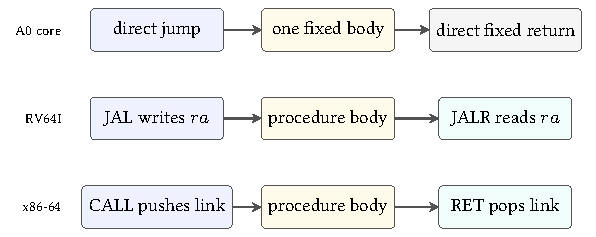
\includegraphics[width=0.94\textwidth]{figures/call-mechanisms}
\caption{Selected call and return mechanisms. The ABI assigns meanings to the
link location, stack pointer, argument, result, and preserved state.}
\figalt{A0 has fixed direct return only, RV64 uses ra as a link register, and x86-64 stores the continuation at the stack pointer.}
\label{fig:call-mechanisms}
\end{figure}

The System V red zone is a further ABI rule: qualifying leaf code may use a
specified region below the current stack pointer without first adjusting
\code{RSP}, subject to the ABI's interruption rule. It is not a general x86-64
hardware property and is not shared by every x86-64 calling convention. This
chapter's worked proof does not rely on it.

\subsection{The ISA supplies effects; the ABI selects a composition}

It is tempting to divide the layers by vocabulary: instructions belong to the
ISA, while register names belong to the ABI. The real boundary is functional.
The ISA defines possible state transitions. The ABI selects some of those
transitions and adds conditions under which separately built components may
compose.

For example, RV64 \code{JAL} can place a link in many destination registers;
the procedure convention commonly selects \code{x1}. An x86-64 near
\code{CALL} has an architectural stack effect, but the ABI determines the
alignment and ownership facts that must hold around it. A direct jump is an
ordinary ISA transfer; it becomes a tail call only when the outgoing argument
state satisfies the next procedure's entry contract and the current
procedure's obligations have already been discharged.

This gives a useful proof order. First apply the instruction rule to establish
the exact link, program-counter, register, and memory effects. Next apply the
ABI lemmas that interpret the affected locations as a continuation, argument,
result, stack area, or preserved resource. Finally apply the procedure theorem
that connects the abstract caller and callee. Reversing that order risks using
the word ``call'' as if it already guaranteed a valid target, valid stack, and
eventual return.

The distinction also explains why an ABI violation need not be an illegal
instruction execution. A body can follow every ISA rule while entering with a
misaligned stack, returning a value in the wrong register, or damaging a
callee-saved register. Architectural validity is necessary for ABI
conformance, but it is not sufficient.

\begin{warning}[title={Name the x86-64 ABI, not merely the ISA}]
System V AMD64 and Microsoft x64 use the same broad instruction set but differ
in argument registers, stack-area rules, and preservation details. A theorem
about one calling convention must not be labeled only ``x86-64.'' Name the ABI
and the selected platform assumptions.
\end{warning}

\section{The same leaf contract in three machines}

Define a mathematical procedure \(I\) that accepts a width-\(w\) word \(x\)
and returns \(x+1\bmod 2^w\). Its boundary contract observes the result,
normal return to the caller's continuation, restored stack pointer, preserved
registers, and all memory outside declared scratch. It permits named volatile
registers and condition state to differ.

The three instances relate their input and result locations:

\begin{table}[htbp]
\centering
\caption{A narrow procedure relation for the add-one leaf examples.}
\begin{tabular}{llll}
\toprule
Machine & Input/result & Continuation & Preserved slice \\
\midrule
A0 fixed case & \(r_0\) & known direct target & \(r_4,r_5,r_6\) \\
RV64 ABI & \code{a0} & \code{ra} & \code{sp}, \code{s0}--\code{s11} \\
SysV AMD64 & \code{RDI}/\code{RAX} & top stack word & \code{RSP}, \code{RBX}, \code{RBP}, \code{R12}--\code{R15} \\
\bottomrule
\end{tabular}
\end{table}

The table is deliberately a slice. The full ABIs classify floating-point,
vector, aggregate, variadic, and memory arguments; define more registers and
process state; and interact with linking and unwind information. A proof of
these leaf examples imports only the rows it uses.

\begin{proofkit}[title={Reader proof for the shared add-one contract}]
Relate the three entry argument words to one arbitrary \(x\). Each body stores
\(x+1\bmod 2^w\) in its declared result location. None writes memory or a
declared preserved data register. A0 reaches its one fixed continuation by a
direct jump. RV64I reads the unchanged incoming \code{ra} in \code{JALR} and
leaves \code{sp} unchanged. x86-64 \code{RET} reads the continuation written
by \code{CALL} and restores \code{RSP} to its pre-call value after consuming
that word. Therefore the related observations agree on result, normal return,
preserved slice, stack restoration, and nonscratch memory.
\end{proofkit}

This proof contains machine-specific premises. The x86-64 case assumes the
return-address load is valid and contains the caller's continuation. The RV64
case assumes \code{ra} names a valid aligned return target under the selected
semantics. The A0 case has only one statically fixed caller. If any premise is
removed, the common mathematical result does not rescue the control claim.

\section{Nested calls and frame preservation}

A nested call makes preservation visible. Suppose a function receives \(x\),
computes an intermediate \(u\), calls another function, and then combines its
result with \(u\). The value \(u\) is live across the call. If it occupies a
volatile register, the caller must save it. If it occupies a callee-saved
register, the current function must restore that register for its own caller
before returning.

\begin{figure}[htbp]
\centering
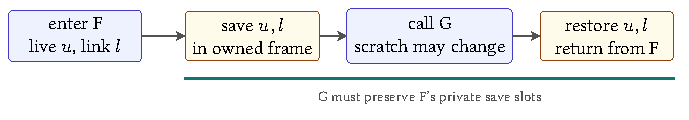
\includegraphics[width=0.82\textwidth]{figures/nested-call-obligations}
\caption{Preservation obligations cross call boundaries. A live intermediate
and the caller's continuation must survive the nested call by declared means.}
\figalt{Caller enters function F, F saves a live value and continuation, calls G, restores them, and returns.}
\label{fig:nested-call-obligations}
\end{figure}

A conventional frame may contain a saved continuation, saved preserved
registers, local objects, spill slots, and outgoing stack arguments. Their
layout is not established merely by drawing boxes. Each slot needs a byte interval;
distinct live objects need disjoint intervals unless sharing is intentional;
each access needs the right width; and the epilogue must load the same saved
values before deallocation.

\begin{proofkit}[title={Preservation by save, call, and restore}]
Let location \(q\) contain entry value \(v\), and suppose the callee may change
\(q\). Before the nested call, store \(v\) in a private frame slot \(m\). The
call may change \(q\) but must not change \(m\) under the nested contract.
After return, load \(m\) into \(q\). The final value of \(q\) is then \(v\).
The proof depends on slot validity, nonaliasing with nested writes, correct
width and byte order, and normal return to the restore instruction.
\end{proofkit}

\subsection{Normal return is only one exit class}

Unwinding after exceptions is harder because the ordinary epilogue may not
run. A procedure may also trap on an invalid access, fail a checked arithmetic
operation, receive an asynchronous signal, diverge, or terminate the process.
Those outcomes cannot be silently folded into a theorem whose conclusion says
that control returns to the saved continuation.

One clean specification partitions behavior. On a normal exit, the result and
ABI preservation clauses hold. On a named exceptional exit, a different
relation describes the transferred control, visible state, and resources that
must remain recoverable. Divergence is a trace property rather than an exit
state. A partial-correctness theorem may say what follows \emph{if} normal
return occurs; a total-correctness theorem must additionally rule out every
other behavior permitted by its model.

Platform unwind metadata and language exception rules provide a route to
recover saved registers and older frames without executing the ordinary
epilogue. The metadata is then part of the binary contract and deserves its
own validation: its description of frame changes must agree with the actual
instructions at each covered program point. Debug information that merely
prints a plausible backtrace is weaker evidence than a checked correspondence
between unwind rows and instruction semantics. Full unwinding remains outside
this first scalar model, but the boundary is now explicit.

Fault ordering also matters. If a prologue adjusts the stack pointer and then
faults while saving a register, the machine is neither at the entry boundary
nor at the normal exit boundary. A proof system that models faults needs the
intermediate state and the architectural rule selecting the reported fault.
If the theorem excludes faults, its precondition must be strong enough to make
every prologue, body, and epilogue access valid.

\section{Observing ABI conformance}

A function need not restore volatile registers, temporary flags, or bytes in
its private frame after release when the contract makes them unobservable. It
must restore the stack pointer and every callee-saved register on normal
return. It must not damage caller-owned memory. The return value must appear in
the declared location, and control must reach the saved continuation.

The rule is observational equivalence with a structured boundary. Two bodies may
use different frame sizes, instruction counts, scratch registers, and internal
control flow while conforming to the same contract. Conversely, identical
return values do not establish conformance if a preserved component differs.

\begin{example}[title={The smallest useful ABI counterexample}]
Run two add-one bodies from related entries. Both return the expected result.
One also replaces a preserved register value 7 with 8. The result-only
observation reports agreement; the ABI observation reports the concrete
register mismatch. Appending a caller that reads that register turns the
boundary failure into a visible program difference.
\end{example}

Tail calls alter the return path. A proper tail transfer may reuse the current
caller's continuation instead of creating another one, but only after the
current frame and preservation obligations have been discharged. Calling a
jump a tail call does not prove that the ABI state at the target is valid.

\section{An introductory Axeyum route}

The present Axeyum checkout still lacks executable A0 and real-ISA procedure
semantics. The appropriate first implementation is therefore a small,
machine-neutral procedure-contract checker layered over future step traces.
It should not begin by encoding an entire platform ABI.

Represent an entry observation, a normal-return observation, input and result
maps, volatile and preserved location sets, stack-pointer checkpoints, owned
memory intervals, and an expected continuation. A trace adapter supplies the
first and last related states. The contract checker compares every promised
component and reports the first mismatch by class.

Then connect one A0 fixed-return trace. Its positive case computes add-one and
preserves the declared slice. Controls change the result, one preserved
register, the final stack pointer, a caller-owned byte, and the continuation.
Every mutation must fail through the corresponding contract clause.

RV64I and x86-64 adapters require source-pinned decoder and step packages
before their traces count as machine-code evidence. RV64 controls should
overwrite \code{ra} across a nested call, omit a saved \code{s} register, or
misalign \code{sp}. x86-64 controls should damage the stacked return address,
restore the wrong \code{RSP}, omit an \code{RBX} restore, or enter a nested
call at the wrong alignment.

\begin{goingdeeper}[title={Contract checking and semantic checking are different}]
A contract checker can prove that two supplied endpoint states satisfy an ABI
relation. It does not prove that instruction bytes generated those endpoints.
A trace checker connects every adjacent state to executable semantics. A
complete evidence route needs both, plus decoder provenance and controls that
fail in each layer.
\end{goingdeeper}

For a solver-backed preservation theorem, symbolically execute the selected
body from arbitrary contract-satisfying inputs and ask whether any promised
exit component can differ. Replay a satisfiable counterexample through the
executable semantics. For an unsatisfiable result, retain the exact formula,
semantic digests, and the strongest available independent evidence. Keep the
theorem limited to the body, ABI slice, memory region, and normal-return path
actually encoded.

\section{Where the procedure model stops}

This chapter covers ordinary scalar calls and normal returns. It excludes
floating-point and vector argument classes, aggregate classification,
variadic functions, structure returns, thread-local state, dynamic linking,
position-independent linkage sequences, system calls, signals, interrupts,
exceptions, unwinding, coroutines, privilege changes, and control-flow
enforcement.

It also excludes stack exhaustion, guard pages, asynchronous modification,
concurrency, and timing. A valid architectural frame can still leak secrets
through access patterns or speculative behavior under a stronger observation.
Those claims require another model.

The narrow result remains powerful. A procedure boundary lets code written at
different times, in different languages, and by different people compose
through a finite agreement. The machine sees words, addresses, and control
transfers. The ABI turns those objects into a promise one component can keep
for another.

\section{Exercises}

\begin{enumerate}
\item Separate ISA facts, assembler spellings, and ABI rules in the RV64I
\code{add_one} listing.

\item Do the same for the x86-64 listing. Include \code{RDI}, \code{RAX},
\code{RSP}, the stacked continuation, and \code{RET}.

\item \textbf{Execute.} Let an x86-64 call begin with \code{RSP=0x1000} and
return address \code{0x402006}. Trace the stack-pointer and return-address
memory effects of the selected near \code{CALL} and matching \code{RET}.

\item Explain why core A0 cannot implement a reusable return through \(r_7\).
State the minimum new semantic capability an extension would need.

\item \textbf{Prove.} For nonwrapping address arithmetic, prove that allocating
and releasing an \(F\)-byte frame restores the entry stack pointer. Then give
three frame errors that this equality does not exclude.

\item For a 32-byte downward-growing frame at entry pointer 256, list its byte
interval. Decide whether 8-byte stores at 224, 248, and 252 stay inside it.

\item Give frame sizes that preserve 16-byte alignment and sizes that break
it. State the checkpoint at which your claim applies.

\item Mark each selected RISC-V ABI register as argument/result, temporary,
preserved, link, or stack pointer: \code{a0}, \code{a7}, \code{t2},
\code{s3}, \code{ra}, and \code{sp}.

\item A live value occupies \code{t0} across a nested RV64 call. Give two
correct preservation strategies and identify who owes each save and restore.

\item \textbf{Break.} Remove the save of incoming \code{ra} from a non-leaf
RV64 function. Construct the shortest trace that returns to the wrong address.

\item Give a System V AMD64 body that returns the right value but violates one
callee-saved-register obligation. Append a caller that observes the damage.

\item Explain why a leaf x86-64 function containing only \code{lea} and
\code{ret} still has a memory-reading return step.

\item \textbf{Transfer.} Write the complete narrow state relation used by the
three add-one examples. Include input, result, continuation, preserved state,
stack state, memory, outcome, and permitted scratch differences.

\item Extend that relation to a nested call with one live intermediate. State
the frame-slot nonaliasing premise needed by the save/restore proof.

\item Design the first procedure-contract artifact for Axeyum. Include
endpoint states, trace reference, observation sets, owned memory, ABI source
pin, and five independently firing negative controls.

\item Distinguish a decoder proof, trace proof, endpoint contract check, and
cross-ISA procedure refinement. Explain what evidence each still lacks.

\item Explain why a tail jump is ABI-correct only after the current function's
frame and preservation obligations have been discharged.
\end{enumerate}
